\documentclass[12pt]{article}
\usepackage[margin=2.5cm]{geometry}
\usepackage{enumerate}
\usepackage{amsfonts}
\usepackage{amsmath}
\usepackage{fancyhdr}
\usepackage{amsmath}
\usepackage{amssymb}
\usepackage{amsthm}
\usepackage{mdframed}
\usepackage{graphicx}
\usepackage{subcaption}
\usepackage{adjustbox}
\usepackage{listings}
\usepackage{xcolor}
\usepackage{booktabs}
\usepackage[utf]{kotex}
\usepackage{hyperref}

\definecolor{codegreen}{rgb}{0,0.6,0}
\definecolor{codegray}{rgb}{0.5,0.5,0.5}
\definecolor{codepurple}{rgb}{0.58,0,0.82}
\definecolor{backcolour}{rgb}{0.95,0.95,0.92}

\lstdefinestyle{mystyle}{
    backgroundcolor=\color{backcolour},
    commentstyle=\color{codegreen},
    keywordstyle=\color{magenta},
    numberstyle=\tiny\color{codegray},
    stringstyle=\color{codepurple},
    basicstyle=\ttfamily\footnotesize,
    breakatwhitespace=false,
    breaklines=true,
    captionpos=b,
    keepspaces=true,
    numbers=left,
    numbersep=5pt,
    showspaces=false,
    showstringspaces=false,
    showtabs=false,
    tabsize=1
}

\lstset{style=mystyle}

\pagestyle{fancy}
\renewcommand{\headrulewidth}{0.4pt}
\lhead{CSC 209}
\rhead{Review 9 Solution}

\begin{document}
\title{CSC 209 Review 9 Solution}
\maketitle

\bigskip

\begin{enumerate}[1.]
    \item

    \begin{enumerate}[a)]
        \item 0

        \bigskip

        \underline{\textbf{Notes}}

        \begin{itemize}
            \item \texttt{a)} is 0 because  (\texttt{i $>>$ 1 + j $>>$ 1 $=$ i $>>$ 10 $>>$ 1 = 0})
            \item
            \textbf{Bitwise Shift Operators}

            \begin{itemize}
                \item has lower precedence than arithematic operators

                \bigskip

                \underline{\textbf{Example:}}

                \bigskip

                \texttt{i $<<$ 2 + 1} means \texttt{i $<<$ (2+1)} and not \texttt{(i $<<$ 2) + 1}

                \bigskip


                \item $<<$ : Left Shift
                \item $>>$ : Right Shift
                \item \textit{Tip:} Always shift only on \underline{unsigned} numbers for portability


                \bigskip

                \underline{\textbf{Example}}

                \bigskip

                \begin{center}
                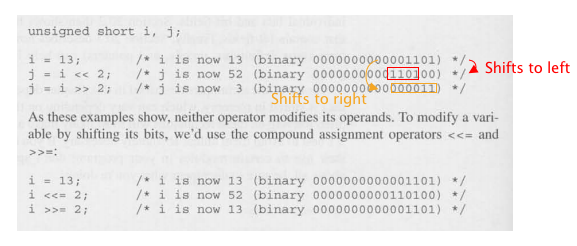
\includegraphics[width=0.9\linewidth]{images/review_9_solution_1.png}
                \end{center}

                \item \texttt{$>>=$} / \texttt{$<<=$} : Are bitwise shift equivalent of \texttt{$+=$}
            \end{itemize}


        \end{itemize}

        \item 0

        \bigskip

        \underline{\textbf{Notes}}

        \begin{itemize}
            \item \texttt{~i} is \texttt{1111111111111111}
            \item \texttt{i} is \texttt{0000000000000000}
            \item so \texttt{~i \& i $=$ 0}
            \item \texttt{~}: Bitwise complement (NOT)

            \bigskip

            \begin{center}
                \begin{tabular}{|c|c|c|}
                    \hline
                    a & $\sim$ a\\
                    \hline
                    0 & 1\\
                    1 & 0\\
                    \hline
                \end{tabular}
            \end{center}

            \bigskip

            \textbf{Example:}

            \bigskip

\begin{lstlisting}[language=c]
    0   1   1   1   //<- this is 7
    --------------
    1   0   0   0   //<- this is 8

    so, ~ 7 = 8
\end{lstlisting}


            \bigskip
            \item \texttt{\&}: Bitwise \textit{and}

            \bigskip

            \begin{center}
                \begin{tabular}{|c|c|c|}
                    \hline
                    a & b & a \& b\\
                    \hline
                    0 & 0  & 0 \\
                    0 & 1  & 1 \\
                    1 & 0  & 0 \\
                    1 & 1  & 1 \\
                    \hline
                \end{tabular}
            \end{center}

            \bigskip

            \textbf{Example:}

            \bigskip

\begin{lstlisting}[language=c]
    0   1   1   1   //<- this is 7
    0   1   0   0   //<- this is 4
    --------------
    0   1   0   0   //<- this is 4

    so, 7 & 4 = 4
\end{lstlisting}

            \bigskip
            \item \texttt{\textrm}: Bitwise \textit{exclusive or}
            \item \texttt{$\vert$}: Bitwise \textit{inclusive or}
        \end{itemize}

        \item 1

        \bigskip

        \underline{\textbf{Notes}}

        \begin{itemize}
            \item \texttt{~i} is \texttt{1111111111111110}
            \item \texttt{j} is \texttt{0000000000000000}
            \item \texttt{~i \& j} is \texttt{0000000000000000} or 1
            \item \texttt{~i \& j \^{} k} is 1
            \item \texttt{\^{}}: Bitwise XOR

            \bigskip

            \begin{center}
                \begin{tabular}{|c|c|c|}
                    \hline
                    a & b & a \^{} b\\
                    \hline
                    0 & 0  & 0 \\
                    0 & 1  & 1 \\
                    1 & 0  & 1 \\
                    1 & 1  & 0 \\
                    \hline
                \end{tabular}
            \end{center}

            \bigskip

            \textbf{Example:}

            \bigskip

    \begin{lstlisting}[language=c]
    0   1   1   1   //<- this is 7
    0   1   0   0   //<- this is 4
    --------------
    0   0   1   1   //<- this is 3

    so, 7 ^ 4 = 3
    \end{lstlisting}
        \end{itemize}

        \item 0

        \bigskip

        \underline{\textbf{Example}}

        \begin{itemize}
            \item \texttt{i} is \texttt{0000000000000111}
            \item \texttt{j} is \texttt{0000000000001000}
            \item \texttt{i \^{} j} is \texttt{0000000000000000} or 0
            \item \texttt{k} is \texttt{0000000000001001}
            \item \texttt{i \^{} j \& k} is \texttt{0000000000000000} or 0
        \end{itemize}

        \bigskip

        \begin{mdframed}
        \underline{\textbf{Correct Solution}}

        \bigskip

        \color{red}15\color{black}
        \end{mdframed}

        \bigskip

        \underline{\textbf{Notes}}

        \begin{itemize}
            \item There is a precendence to the order of operations

            \begin{center}
            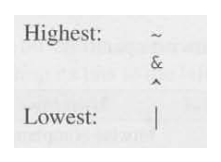
\includegraphics[width=0.4\linewidth]{images/review_9_solution_2.png}
            \end{center}
        \end{itemize}
    \end{enumerate}

\end{enumerate}

\end{document}